\documentclass[journal]{IEEEtran}

\usepackage{circuitikz}   
\usepackage{tikz}
\usepackage[spanish, es-noshorthands]{babel}
\usepackage{float}
\usepackage{instructivo}
\usepackage{tabularx}
\usepackage{array}
\newcolumntype{Y}{>{\raggedright\arraybackslash}X}
\graphicspath{{./}{./fig/}}
\usepackage[natbib=true,style=trad-unsrt,backend=biber]{biblatex}
\addbibresource{literatura.bib}

\hyphenation{op-tical net-works semi-conduc-tor}

\usepackage{amsmath}
\usetikzlibrary{shapes, arrows.meta, positioning, calc}
 
% --- Estilos ---
\tikzset{
  block/.style={
    draw, rectangle,
    minimum width=3.2cm, minimum height=1.2cm,
    align=center, font=\small
  },
  line/.style={draw, -{Latex[length=2.5mm, width=2mm]}},
  siglabel/.style={font=\footnotesize, text=blue!65!black},
  blklabel/.style={font=\footnotesize, right=0.15cm, text=black}
}

\begin{document}
\setlength{\parindent}{4.2mm}
\title{Parcial 1 Control Automático}

\author{Matías~A.~Camacho,~\IEEEmembership{Estudiante,~TEC}
        y~Juan~P.~Elizondo,~\IEEEmembership{Estudiante,~TEC}
}

% The paper headers
\markboth{Laboratorio de control automático, IIS2026}%
{Laboratorio de control automático}


% make the title area
\maketitle


%%%%%%%%%%%%%%%%%%%%%%%%%%%%%%%%%%%%%%%%%%%%%%%%%%%%%%%%%%%%%%%%%%%%%%%%%%%%%%%%%%%%%%%%%%%%%%
%%%%%%%%%%%%%%%%%%%%%%%%%%%%%%%%%%%%%%%%%%%%%%%%%%%%%%%%%%%%%%%%%%%%%%%%%%%%%%%%%%%%%%%%%%%%%%
\section{Introducción}

\IEEEPARstart{E}{l} presente trabajo aborda el diseño de compensadores y controladores clásicos para dos sistemas realimentados. En el primer problema se diseña un compensador en atraso (lag) para mejorar el error en régimen permanente ante una entrada rampa. En el segundo, se diseña y compara un controlador PID (o alguna de sus simplificaciones) frente a una red de compensación, para una planta de tercer orden sujeta a especificaciones de tiempo de asentamiento, sobreimpulso y error nulo en estado estacionario. En ambos casos se presentan los resultados intermedios (lugar de las raíces, ecuaciones características) que sustentan las decisiones de diseño.

\section{Problema 1}
En este ejercicio se presenta un sistema, con una planta cuya función de transferencia
es la que se describe en la ecuación \eqref{eq:Planta_1}.

\begin{equation}
        \begin{aligned}
                G_p(s)=\frac{K}{s(s+5)}
        \end{aligned}
\label{eq:Planta_1}
\end{equation}

Además, se está ante un sistema de lazo cerrado con realimentación unitaria. Que con el valor actual
de la ganancia $K$, presenta un $\%OS = 12\%$. Con esta información, resulta importante determinar el valor
de dicha ganancia antes de efectuar cualquier cálculo o diseño sobre el sistema.

Con el porcentaje de sobreimpulso dado, se puede determinar el factor de amortiguamiento $\zeta$ 
mediante la ecuación \eqref{eq:Zeta_Planta_1}, según se muestra:

\begin{equation}
        \begin{aligned}
                \zeta &= \frac{-\ln(\frac{\%OS}{100})}{\sqrt{\pi^2+\ln^2(\frac{\%OS}{100})}} \\
                \zeta &= 0.559 \\
        \end{aligned}
\label{eq:Zeta_Planta_1}
\end{equation}


Por definición, la función de transferencia en lazo cerrado, que describe a este sistema,
está dada de la siguiente manera:


\begin{equation}
        \begin{aligned}
                T(s) &= \frac{G_p(s)}{1+H(s)G_p(s)} \\
                     &= \frac{K}{s^2+5s+K} \\
        \end{aligned}
\label{eq:Planta_1_lazo_cerrado}
\end{equation}

Con esto, y por tratarse de un sistema de segundo orden, es posible determinar 
la frecuencia natural $\omega_n$ mediante la ecuación \eqref{eq:Omega_n_Planta_1}.

\begin{equation}
        \begin{aligned}
                2\zeta\omega_n &= 5 \\
                \omega_n &= 4.4689 \\
        \end{aligned}
\label{eq:Omega_n_Planta_1}
\end{equation}

Con el valor de $\omega_n$ determinado, es posible calcular el valor de la ganancia $K$ al analizar la
Ecuación~\eqref{eq:Planta_1_lazo_cerrado}, el cual da un valor de $K = 19.97$, redondeado, $K = 20$.

\subsection{Error de régimen permanente con el sistema sin compensar}
Para este caso, se solicita determinar el error ante una entrada tipo rampa. Cabe mencionar
que este mismo error ante una entrada tipo escalón es nulo, al tratarse de un sistema de tipo 1 (con un integrador puro).
La constante de error para una entrada tipo rampa, $K_v$, se determina de la siguiente forma:

\begin{equation}
        \begin{aligned}
                K_v &= \lim_{s\to 0} sG_p(s) \\
                K_v &= \lim_{s\to 0} s\frac{K}{s(s+5)} \\
                K_v &= \lim_{s\to 0} \frac{K}{s+5} \\
                K_v &= \frac{20}{5} = 4
        \end{aligned}
\label{eq:Kv_Planta_1}
\end{equation}

Posteriormente, el error en régimen permanente, corresponde al inverso de la constante $K_v$:

\begin{equation}
        \begin{aligned}
                e_{ss}(\infty) &= \frac{1}{K_v} \\
                e_{ss}(\infty) &= \frac{1}{4} = 0.25
        \end{aligned}
\label{eq:Error_Planta_1}
\end{equation}

Como se evidencia en el resultado obtenido anteriormente, ante una entrada tipo rampa unitaria, el
sistema no es capaz de lograr un error nulo, por lo que la respuesta tendrá una forma similar al de una 
rampa unitaria, pero sin ser exactamente igual, según se muestra en la Figura~\ref{fig:Ej1_respuesta_sinCompensar}; además, 
la evolución del error a lo largo del tiempo, se muestra en la Figura~\ref{fig:Ej1_error_sinCompensar}.

\begin{figure}[H]
        \centering
        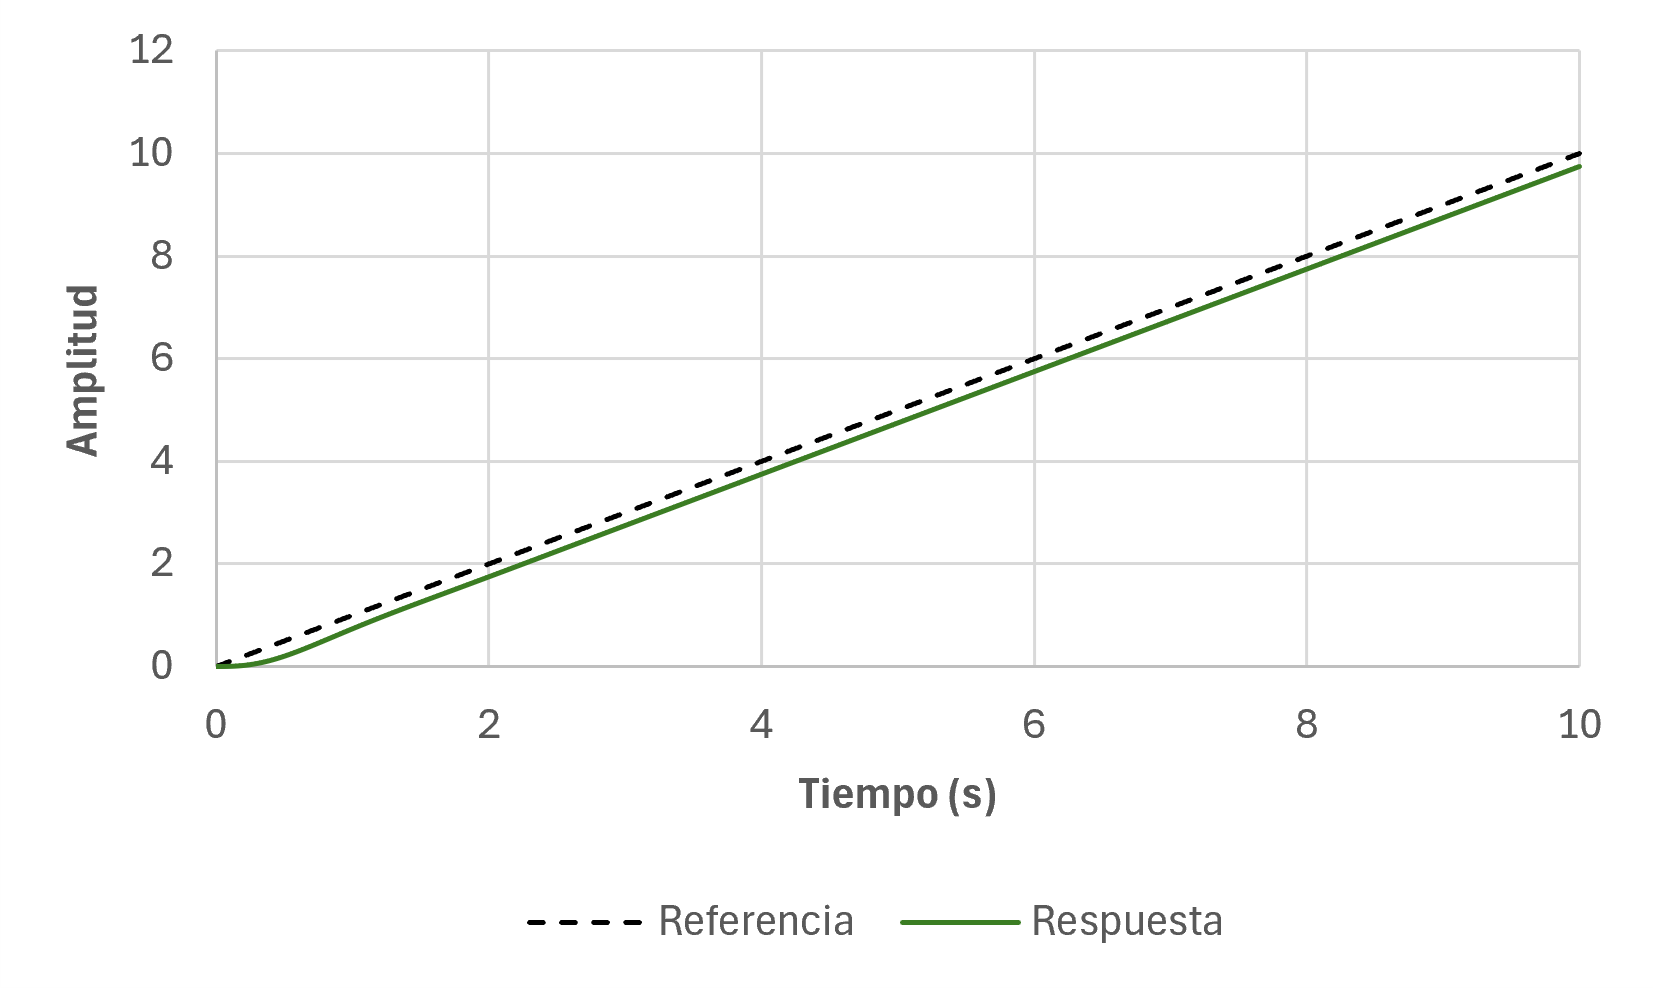
\includegraphics[width=\linewidth]{Ej1_respuesta_sin_compensador.png}
        \caption{Respuesta del sistema sin compensar, ante una entrada tipo rampa unitaria.}
        \label{fig:Ej1_respuesta_sinCompensar}
\end{figure}

\begin{figure}[H]
        \centering
        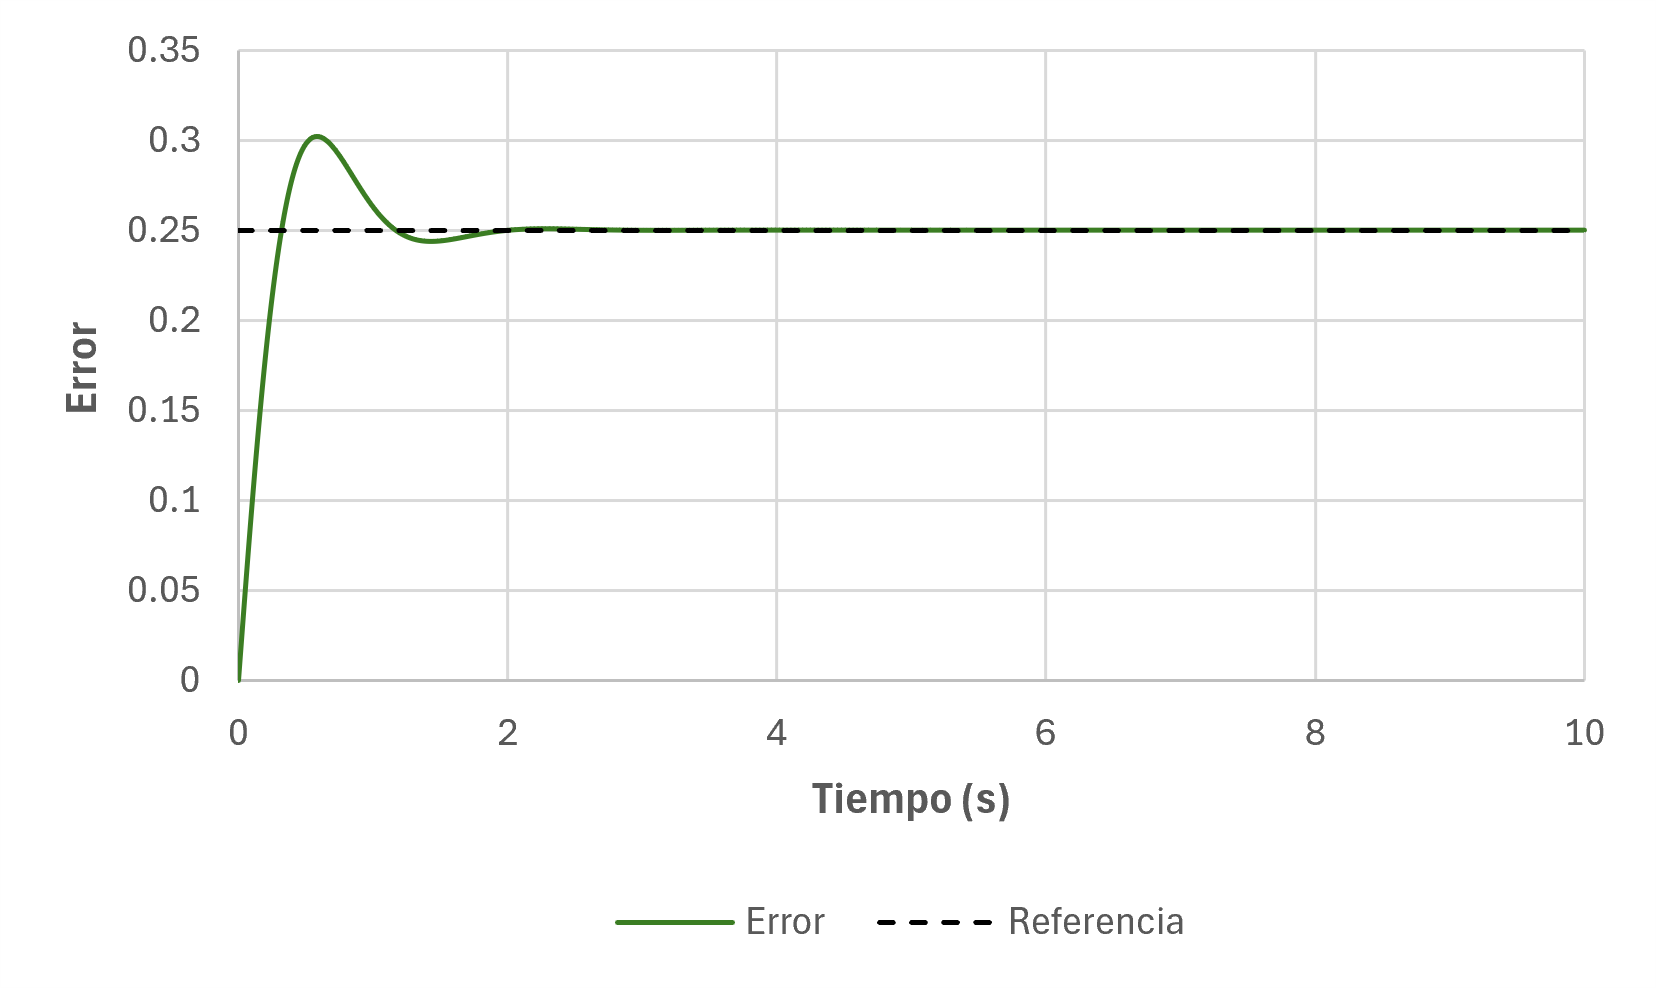
\includegraphics[width=\linewidth]{Ej1_error_sin_compensador.png}
        \caption{Evolución del error del sistema sin compensar, ante una entrada tipo rampa unitaria.}
        \label{fig:Ej1_error_sinCompensar}
\end{figure}

\subsection{Diseño de un compensador en atraso (lag)}
Con la finalidad de solucionar el problema que presenta el sistema, al no poder lograr un error nulo en estado
estacionario solo con un compensador proporcional, se solicita el diseño de un compensador de atraso (tipo lag),
que logre reducir el error en un factor de 15.

Para diseñarlo, se parte por determinar la cantidad de error deaseada, al disminuirse por un factor
de 15, este es:

\begin{equation}
        \begin{aligned}
                e_{ss,~C}(\infty) &= \frac{0.25}{15} = \frac{1}{60} \approx 0.0167
        \end{aligned}
\label{eq:Error_Planta_1_compensada}
\end{equation}

Con lo cual, la nueva constante de error, $K_v$, corresponde a:

\begin{equation}
        \begin{aligned}
                K_v &= \frac{1}{e_{ss,~C}(\infty)} = 60
        \end{aligned}
\label{eq:Kv_Planta_1_compensada}
\end{equation}

Posteriormente, se sabe que la constante de error $K_v$, también se puede calcular mediante la multiplicación
de la ganancia del sistema, $K$, por la magnitud de cada uno de los ceros, dividido entre la multiplicación
de la magnitud de cada uno de los polos. Además, al agregar el compensador de atraso, se le suma a esta multiplicación
la magnitud del cero y del polo del compensador (Ecuación~\eqref{eq:Kv_Planta_1_compensada_2}).

\begin{equation}
        \begin{aligned}
                K_v &= \frac{K \cdot z_c \cdot z_1 \cdot z_2~...}{p_c \cdot p_1 \cdot p_2~...} \\
        \end{aligned}
\label{eq:Kv_Planta_1_compensada_2}
\end{equation}

Al analizar estos dos escenario, y considerando que la ganancia proporcional, $K$, es igual en ambos casos.
Se puede establecer la siguiente relación:

\begin{equation}
        \begin{aligned}
                \frac{K_{v_N}}{K_{v_O}} &= \frac{z_c}{p_c} \\
        \end{aligned}
\label{eq:Kv_Planta_1_compensada_3}
\end{equation}

Con lo cual, al escoger una ubicacion arbitraria para el polo del compensador en $\sigma = -0.01$,
se obtiene que el cero del compensador debe ubicarse en $\sigma = -0.15$, para cumplir con la relación
de la ecuación \eqref{eq:Kv_Planta_1_compensada_3}. 
Por lo que la función de transferencia del compensador de atraso (lag) es la siguiente:

\begin{equation}
        \begin{aligned}
                C_{lag}(s) &= \frac{s+0.15}{s+0.01} \\
        \end{aligned}
\label{eq:Compensador_Planta_1}
\end{equation}

Finalmente, en la Figura~\ref{fig:Ej1_respuesta_conCompensador}, se muestra la respuesta del sistema compensado, 
ante una entrada tipo rampa unitaria. Mientras que la evolución del error del sistema ya compensado, se muestra en 
la Figura~\ref{fig:Ej1_error_conCompensador}.

\begin{figure}[H]
        \centering
        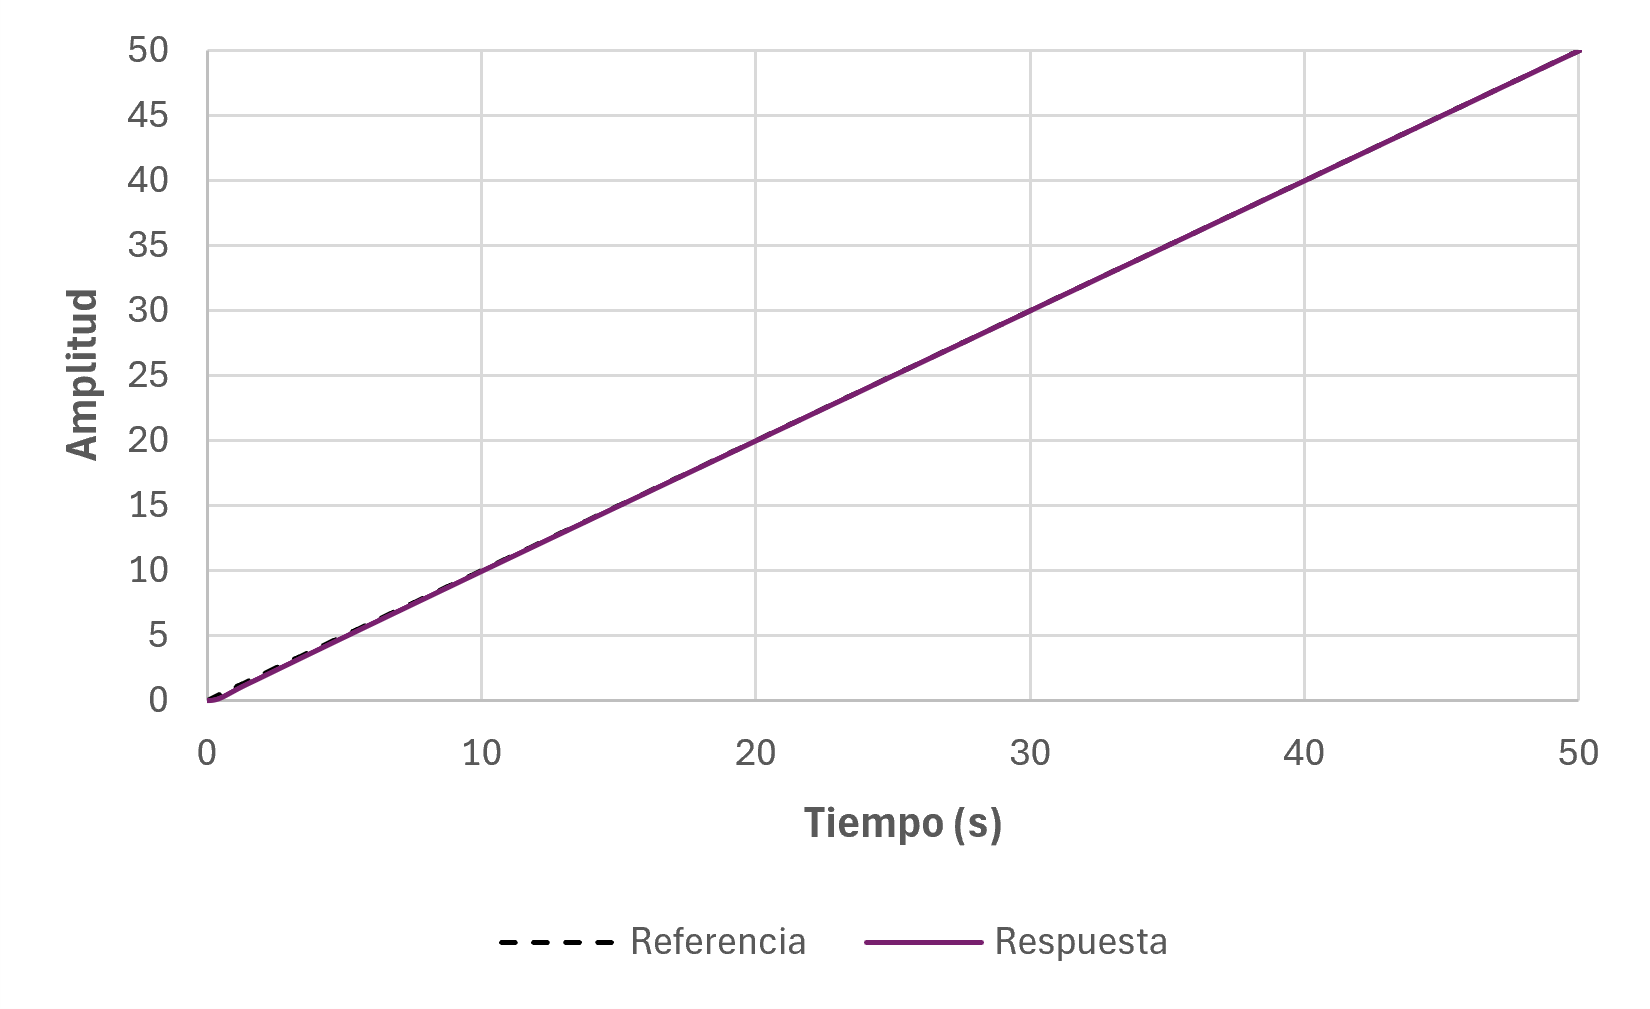
\includegraphics[width=\linewidth]{Ej1_respuesta_con_compensador.png}
        \caption{Respuesta del sistema compensado, ante una entrada tipo rampa unitaria.}
        \label{fig:Ej1_respuesta_conCompensador}
\end{figure}

\subsection{Error de régimen permanente con el sistema compensado}
El valor de error en régimen permanente del sistema con el compensador ya implementado, 
se calcula primero obteniendo la constante de error mediante la ecuación~\eqref{eq:Kv_Planta_1_compensada_2}:

\begin{equation}
        \begin{aligned}
                K_v &= \frac{20 \cdot 0.15}{0.01 \cdot 5} = 60 \\
        \end{aligned}
\label{eq:Kv_Planta_1_compensada_4}
\end{equation}

con lo que se obtiene un error en régimen permanente de $e_{ss,~C}(\infty) \approx 0.0167$. El cual
concuerda perfectamente con el obtenido en la ecuación~\eqref{eq:Error_Planta_1_compensada}.

\begin{figure}[H]
        \centering
        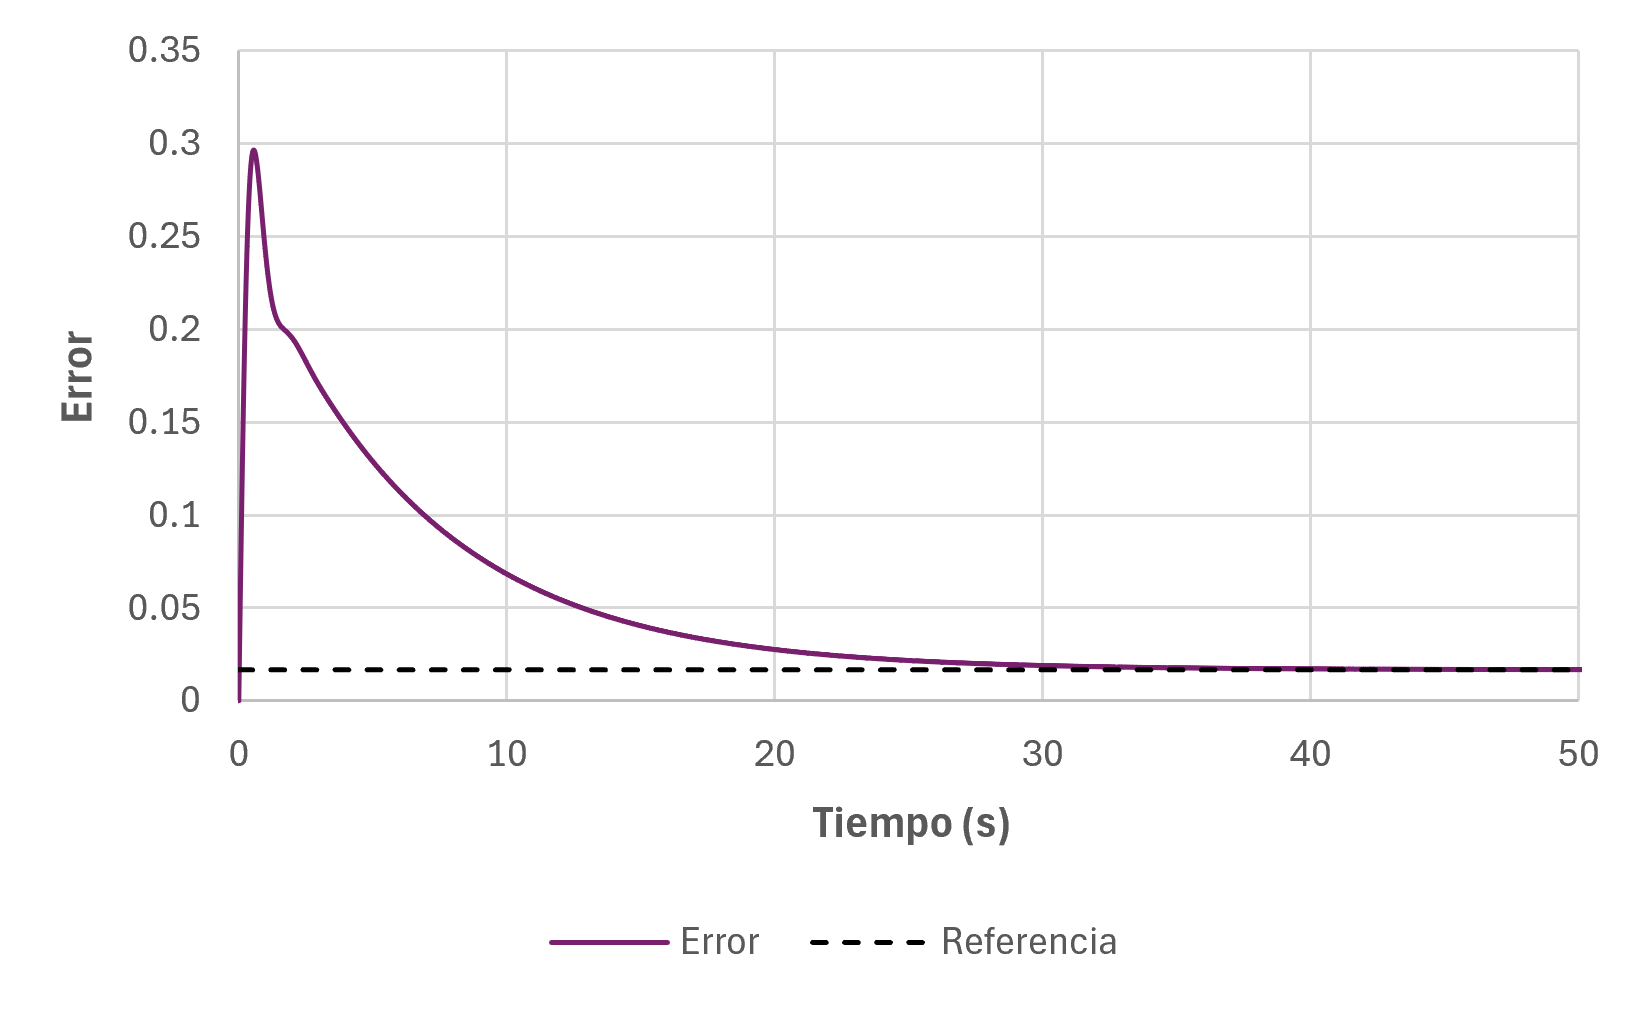
\includegraphics[width=\linewidth]{Ej1_error_con_compensador.png}
        \caption{Evolución del error del sistema compensado, ante una entrada tipo rampa unitaria.}
        \label{fig:Ej1_error_conCompensador}
\end{figure}

\subsection{Evaluación de mejora}
En términos generales, y por la forma en la que se diseñó el compensador de atraso. Este logra cumplir con lo deseado, 
reduciendo el error en régimen permanente en un factor de 15. Esto equivale a que el error final corresponda únicamente 
al $6.67\%$ del error original, es decir, una reducción porcentual del $93.33\%$ aproximadamente.
Todo esto se puede verificar fácilmente al comparar la Figura~\ref{fig:Ej1_error_sinCompensar}, contra la Figura~\ref{fig:Ej1_error_conCompensador}.


\section{Problema 2}
Se consideró la siguiente planta de tercer orden, teniendo en cuenta que tiene realimentación de \mbox{$H(s)=0.2$}.

\begin{equation}\label{eq:Planta}
G_p(s)=\frac{10(s+2)}{(s+1)(s+4)(s+8)}
\end{equation}

\begin{table}[H]
        \centering
        \caption{Características de la respuesta transitoria de la planta sin compensación}
        \label{tab:caracteristicas-respuesta-noncomp}
        \begin{tabular}{lc}
                \hline
                \textbf{Parámetro} & \textbf{Valor} \\
                \hline
                Tiempo de subida       & 1.8895 s \\
                Tiempo transitorio  & 3.6401 s \\
                Tiempo de asentamiento   & 3.6401 s \\
                Mínimo de asentamiento    & 0.5628  \\
                Máximo de asentamiento    & 0.6241  \\
                Sobreimpulso      & 0\% \\
                Subimpulso     & 0\% \\
                Pico           & 0.6241  \\
                Tiempo pico       & 6.3206 s \\
                \hline
        \end{tabular}
\end{table}

\begin{figure}[H]
        \centering
        \includegraphics[width=\linewidth]{nonComp.png}
        \caption{Respuesta de la planta sin compensación.}
        \label{fig:nonComp}
\end{figure}


\subsection{Compensación PID}

Se determinó una región admisible para los polos dominantes de lazo cerrado a partir de las especificaciones de sobreimpulso ($M_p \le 10\%$) y tiempo de asentamiento ($t_s \le 0.8$ s, criterio del 2\%):

\begin{equation}\label{eq:zeta}
\zeta \ge \frac{-\ln(M_p)}{\sqrt{\pi^2+\ln^2(M_p)}} \approx 0.591
\end{equation}

\begin{equation}\label{eq:zetawn}
t_s \approx \frac{4}{\zeta\omega_n} \le 0.8\text{ s} \;\Rightarrow\; \zeta\omega_n \ge 5
\end{equation}

La condición de sobreimpulso fija un valor mínimo de amortiguamiento, mientras que la condición de tiempo de asentamiento fija un valor mínimo para la magnitud de la parte real de los polos dominantes. Ambas restricciones definen una región admisible en el semiplano izquierdo del plano $s$, cuyo vértice teórico se ubica aproximadamente en $-5\pm j6.8$.

Se propuso un controlador PID en la forma

\begin{equation}\label{eq:PID-generico}
C(s)=\frac{K(s+z_1)(s+z_2)}{s}
\end{equation}

\noindent El polo en el origen corresponde a la acción integral pura del PID; su presencia es necesaria porque la realimentación del sistema es $H(s)=0.2\ne1$, y sin acción integral el error de estado estacionario ante entrada escalón sería finito y no nulo, lo cual viola una especificación explícita del problema.

La ubicación de los ceros del controlador se ajustó de forma gráfica utilizando la herramienta \textit{Root Locus Designer} de MATLAB, desplazando iterativamente los ceros hasta que las ramas del lugar de las raíces, dentro de la región admisible definida por las ecuaciones \eqref{eq:zeta}--\eqref{eq:zetawn}, produjeran una respuesta que cumpliera ambas especificaciones. Este procedimiento gráfico convergió a $z_1=15.87$ y $z_2=17.89$, con una ganancia $K=208.82$ obtenida automáticamente por la herramienta mediante la condición de magnitud del lugar de las raíces en el punto de cruce seleccionado.

\begin{equation}\label{eq:Controlador}
C(s)=\frac{208.82(s+15.87)(s+17.89)}{s}
\end{equation}

A diferencia de lo anticipado por el vértice teórico de la región admisible (que corresponde a un par de polos complejos conjugados), la verificación numérica de los polos de lazo cerrado mediante \texttt{damp} mostró que, para este controlador, todos los polos resultan reales:

\begin{equation}
\begin{aligned}
s_1&=-2.0003,\qquad s_2=-14.9049,\\
s_3&=-20.2195,\qquad s_4=-393.52.
\end{aligned}
\end{equation}

Esto corresponde a una respuesta sobre-amortiguada, lo cual es consistente con el bajo sobreimpulso obtenido (Tabla \ref{tab:caracteristicas-respuesta}) y sigue satisfaciendo ampliamente ambas especificaciones de diseño.

Se observa además que $s_1\approx-2.0003$ coincide casi exactamente con el cero de la planta $z_p=-2$ (ecuación \eqref{eq:Planta}). En la función de transferencia de lazo cerrado

\begin{equation}
\small
T(s)=\frac{2088.2\,(s+15.87)(s+17.89)(s+2)}
{(s+393.5)(s+20.22)(s+14.9)(s+2.0003)}
\end{equation}

este par polo--cero prácticamente se cancela, por lo que dicho modo, aunque es el más cercano al eje imaginario, no domina la respuesta transitoria. Esto se confirma al comparar con la aproximación de segundo orden que predeciría el siguiente polo más lento ($s_2=-14.9049$, que daría $t_s\approx4/14.9\approx0.268$~s): el tiempo de asentamiento real obtenido por simulación ($t_s=0.0486$~s) es considerablemente menor, lo que indica que ningún polo individual domina de forma clara la dinámica del sistema compensado, sino que la respuesta resulta de la combinación de los tres polos rápidos remanentes. Por ello, el cumplimiento de las especificaciones se verificó mediante simulación directa (Tabla \ref{tab:caracteristicas-respuesta} y Figura \ref{fig:PIDComp}), en lugar de mediante una aproximación analítica de polo dominante.

\begin{table}[H]
        \centering
        \caption{Características de la respuesta transitoria}
        \label{tab:caracteristicas-respuesta}
        \begin{tabular}{lc}
                \hline
                \textbf{Parámetro} & \textbf{Valor} \\
                \hline
                Tiempo de subida       & 0.0046 s \\
                Tiempo transitorio  & 0.0486 s \\
                Tiempo de asentamiento   & 0.0486 s \\
                Mínimo de asentamiento    & 4.5205 \\
                Máximo de asentamiento    & 5.2140\\
                Sobreimpulso      & 4.2790\% \\
                Subimpulso     & 0\% \\
                Pico           & 5.2140\\
                Tiempo pico       & 0.0151 s \\
                \hline
        \end{tabular}
\end{table}

\begin{figure}[H]
        \centering
        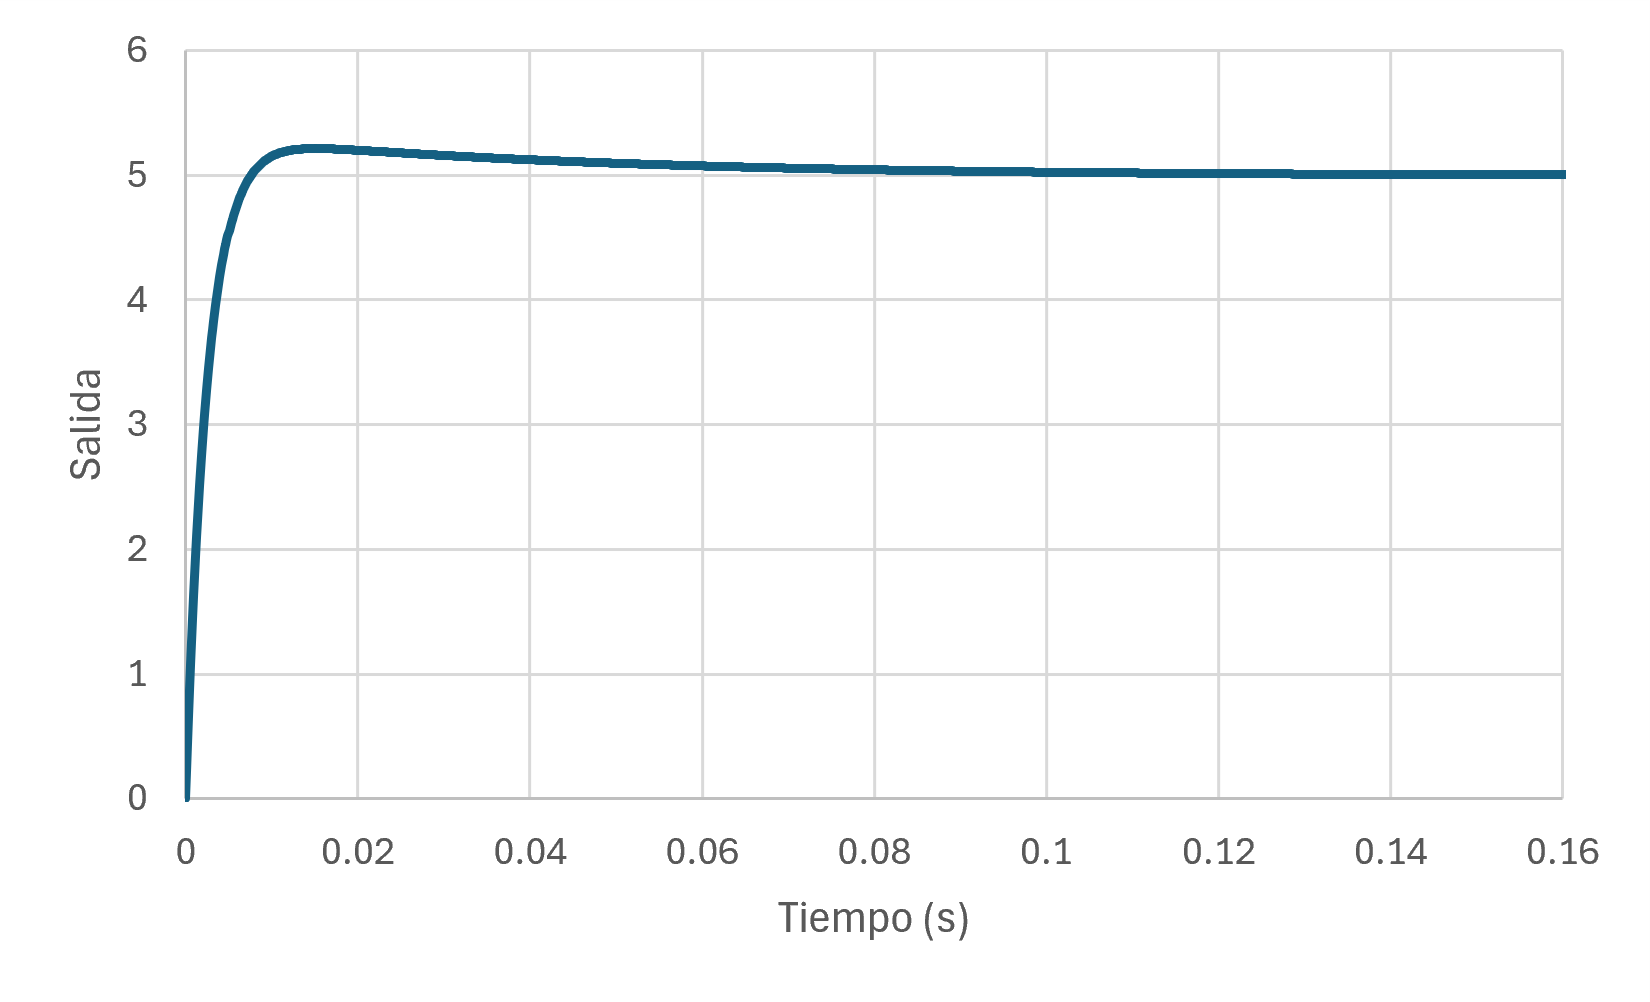
\includegraphics[width=\linewidth]{PIDComp.png}
        \caption{Respuesta de la planta con compensación.}
        \label{fig:PIDComp}
\end{figure}

Viéndose la figura \ref{fig:nonComp}, se aprecia que esta nunca llega al valor estacionario esperado, 5, sino que alcanza un máximo de 0.624. Nótese que el valor final de 5 es debido a que la realimentación no es unitaria, sino de 0.2.

\subsection{Compensación adelanto, atraso o adelantoatraso}

\printbibliography

%%%%%%%%%%%%%%%%%%%%%%%%%%%%%%%%%%%%%%%%%%%%%%%%%%%%%%%%%%%%%%%%%%%%%%%%%%%%%%%%%%%%
%%%%%%%%%%%%%%%%%%%%%%%%%%%%%%%%%%%%%%%%%%%%%%%%%%%%%%%%%%%%%%%%%%%%%%%%%%%%%%%%%%%%


\end{document}